\documentclass{article}
    % General document formatting
    \usepackage[margin=0.7in]{geometry}
    \usepackage{amsthm}
    \usepackage[parfill]{parskip}
    \usepackage[utf8]{inputenc}
    \usepackage{cancel}
    \usepackage{graphicx}
    \graphicspath{./skitser/}
    % Related to math
    \usepackage{amsmath,amssymb,amsfonts,amsthm}

\makeatletter
\newenvironment{proofw}{\par
  \pushQED{\qed}%
  \normalfont \topsep6\p@\@plus6\p@\relax
  \trivlist
  \item[]\ignorespaces
}{%
  \popQED\endtrivlist\@endpefalse
}
\makeatother

\begin{document}

\section{Vektorer og trigonometri}

\subsection{Bevis}

\begin{proofw}
    
Betragt figur \ref{fig:trekant_vektor}, hvor en vinkel $v$ er udspændt af vektoren $\vec{x}$ og $\vec{y}$.

\begin{figure}[h]
    \centering
    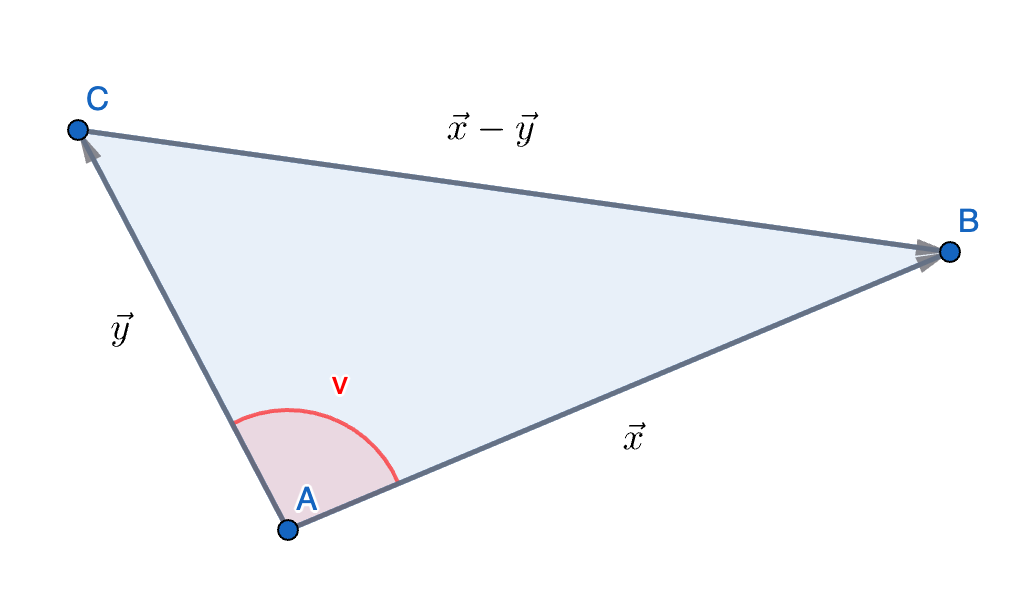
\includegraphics[scale=0.3]{./skitser/trekant_vektor_skitse.png}
    \label{fig:trekant_vektor}
    \caption{Vinkel udspændt af 2 vektorer.}
\end{figure}

Vha. af disse vektorer kan vi danne en trekant, hvori vi kan anvende cosinusrelationerne
til at lave et generelt udtryk for vinklen udspændt af 2 vektorer.
Her kan vi lave et udtryk for den lange side ved at anvende indskudsreglen:

\begin{align*}
    \vec{AB}+\vec{BC}&=\vec{AC}
    \\
    &\Downarrow
    \\
    \vec{BC}&=\vec{AC}-\vec{AB}
    \\
    &\Downarrow
    \\
    \vec{CB}&=-\vec{BC}=\vec{AB}-\vec{AC}
\end{align*}

Så den trejde side noteres $\vec{x}-\vec{y}$, og vi anvender cosinusrelationen, der siger, at i en trekant, så:

$$
    c^2=a^2+b^2-2ab \cdot \cos(v)
$$

Hvilket i vores tilfælde betyder:

$$
    |\vec{x}-\vec{y}|^2=|\vec{x}|^2+|\vec{y}|^2-2|\vec{x}||\vec{y}| \cdot \cos(v)
$$

Nu anvendes det, at $|\vec{x}|^2=\vec{x} \cdot \vec{x}$, det betyder for vores vektor:

$$
    |\vec{x}-\vec{y}|^2=(\vec{x}-\vec{y})\cdot (\vec{x}-\vec{y})
    =|\vec{x}|^2+|\vec{y}|^2-2 \cdot \vec{x}\cdot \vec{y}
$$

Det indsættes i ovenstående:

$$
\cancel{|\vec{x}|^2+|\vec{y}|^2-2} \cdot \vec{x}\cdot \vec{y}
=\cancel{|\vec{x}|^2+|\vec{y}|^2-2}|\vec{x}||\vec{y}| \cdot \cos(v)
$$

Hvor $\cos(v)$ isoleres:

$$
    \cos(v)=\frac{
        \vec{x} \cdot \vec{y}
    }{
        |\vec{x}||\vec{y}|
    }
$$
\end{proofw}

\pagebreak

\section{Vektorer og linjer i planen}

\subsection{Bevis af linjens parameterfremstilling}

\begin{proofw}
    Betragt følgende skitse:
    \begin{figure}[h]
        \centering
        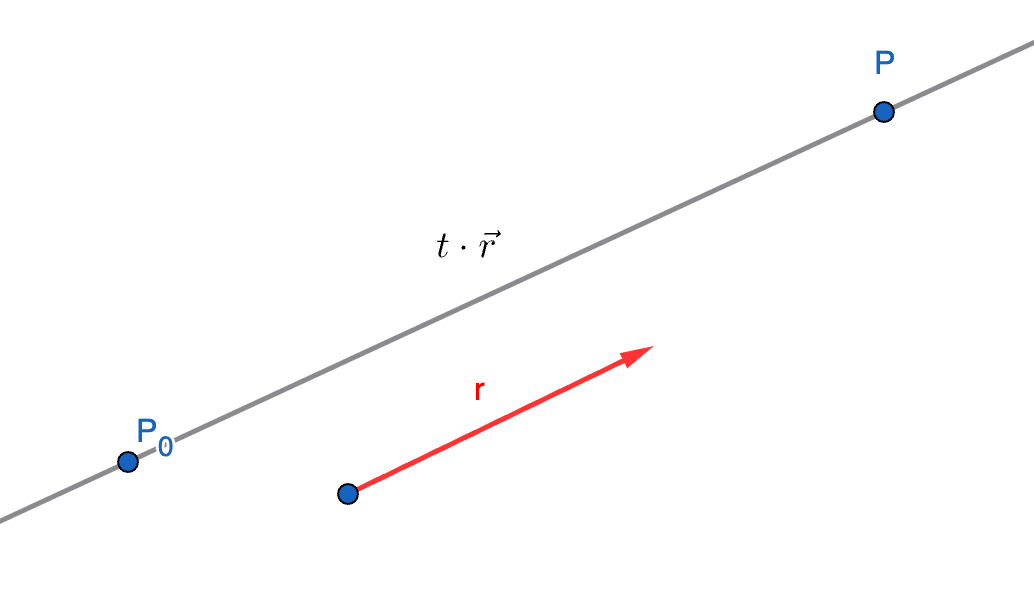
\includegraphics[scale=0.4]{skitser/linje_parameter.png}
    \end{figure}

Tager vi afsæt i punktet $P_0(x_0,y_0)$, hvis position kan beskrives
med vektoren $\vec{OP}$. Tager vi et skridt langs en vektor, der er parallel med linjen,
så vil vores nye position også være på linjen.
Derfor må vi ved at gange retningsvektoren med et vilkårligt tal
kunne ramme alle punkter på linjen.
Så kan vi beskrive vektoren til punktet $P(x,y)$
som vektoren til $P_0$ plus retningsvektoren skaleret:

$$
\vec{OP}=\vec{OP_0}+t\cdot \vec{r}
$$

Vi opsplitter $\vec{OP}$ i $\begin{pmatrix}
    x \\ y
\end{pmatrix}$ og $\vec{r}$ i $\begin{pmatrix}
    r_1 \\ r_2
\end{pmatrix}$:

$$
\begin{pmatrix}
    x
    \\
    y
\end{pmatrix}
=\begin{pmatrix}
    x_0
    \\
    y_0
\end{pmatrix}
+
t \cdot \begin{pmatrix}
    r_1
    \\
    r_2
\end{pmatrix}
$$
\end{proofw}

\subsection{Bevis af linjens ligning}

\begin{proofw}
    Betragt nedenstående figur:
    \begin{figure}[h]
        \centering
        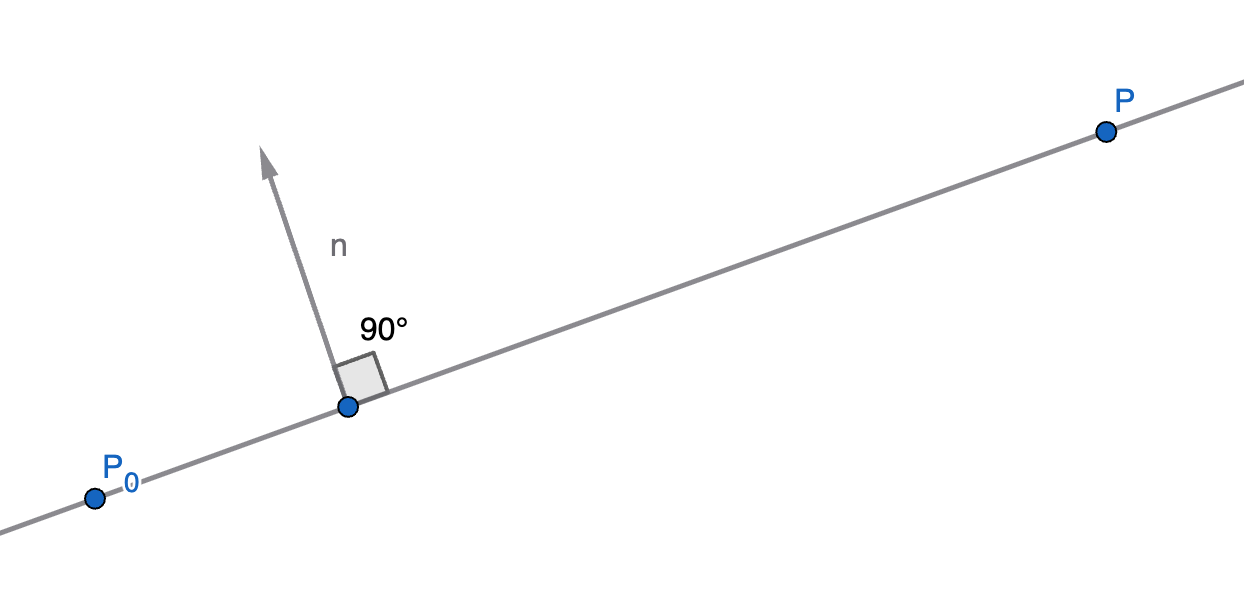
\includegraphics[scale=0.4]{skitser/linjens_ligning.png}
    \end{figure}

    Vi kender $P_0(x_0,y_0)$ og normalvektoren $\vec{n}=\begin{pmatrix}
        a \\ b
    \end{pmatrix}$, $P(x,y)$ er et vilkårligt punkt langs linjen, som vi vil beskrive.
    Vi kan lave en ortogonal vektor til $\vec{n}$ ved at lave vektoren $\vec{P_0P}=\begin{pmatrix}
        x-x_0
        \\
        y-y_0
    \end{pmatrix}$.
    Tricket er så, at vi har 2 ortogonale vektorer, hvilket betyder,
    at deres skalarprodukt er 0, derved kan vi opstille følgende udtryk, hvor $x$ og $y$ alle er punkter på linjen:

    \begin{align*}
        \vec{P_0P}&\cdot\vec{n}=0
        \\
        &\Downarrow
        \\
        \begin{pmatrix}
            x-x_0
            \\
            y-y_0
        \end{pmatrix}
        &\cdot
        \begin{pmatrix}
            a \\
            b
        \end{pmatrix}=0
        \\
        \Downarrow
        \\
        a(x-x_0)&+b(y-y_0)=0
        \\
        \Downarrow
        \\
        ax+by+&(-ax_0-by_0)=0
        \\
        \Downarrow
        \\
        ax+by&+c=0
    \end{align*}

    Det er vist, at en linje kan beskrives ud fra et punkt og en normalvektor til linjen.

\end{proofw}

\end{document}
